% This file was created with tikzplotlib v0.10.1.
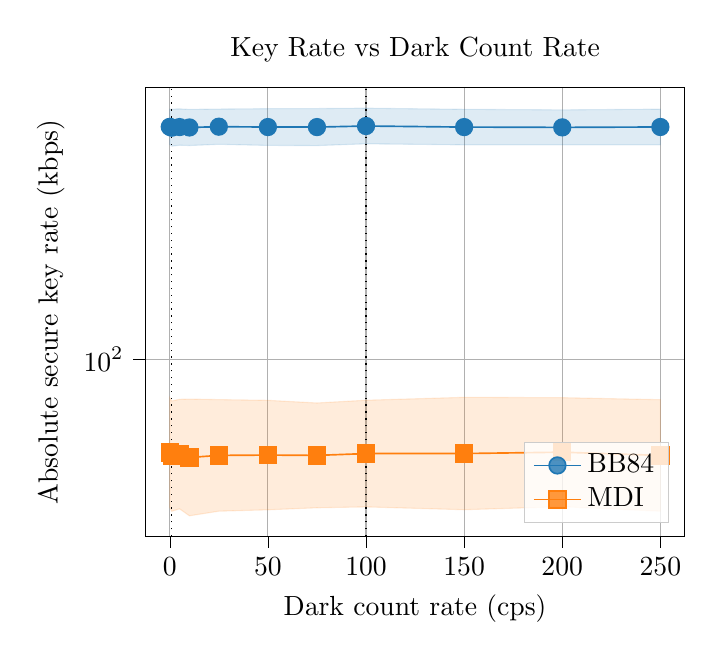
\begin{tikzpicture}
\definecolor{darkgray176}{RGB}{176,176,176}
\definecolor{darkorange25512714}{RGB}{255,127,14}
\definecolor{darkred}{RGB}{139,0,0}
\definecolor{dimgray}{RGB}{105,105,105}
\definecolor{lightgray204}{RGB}{204,204,204}
\definecolor{steelblue31119180}{RGB}{31,119,180}
\begin{axis}[
title={Key Rate vs Dark Count Rate},
legend cell align={left},
legend style={
  fill opacity=0.8,
  draw opacity=1,
  text opacity=1,
  at={(0.97,0.03)},
  anchor=south east,
  draw=lightgray204
},
log basis y={10},
tick align=outside,
tick pos=left,
x grid style={darkgray176},
xlabel={Dark count rate (cps)},
xmajorgrids,
xmin=-12.5, xmax=262.5,
xtick style={color=black},
xtick={-50,0,50,100,150,200,250,300},
xticklabels={
  \(\displaystyle {\ensuremath{-}50}\),
  \(\displaystyle {0}\),
  \(\displaystyle {50}\),
  \(\displaystyle {100}\),
  \(\displaystyle {150}\),
  \(\displaystyle {200}\),
  \(\displaystyle {250}\),
  \(\displaystyle {300}\)
},
y grid style={darkgray176},
ylabel={Absolute secure key rate (kbps)},
ymajorgrids,
ymin=41.0592389323082, ymax=391.864103025714,
ymode=log,
ytick style={color=black},
ytick={1,10,100,1000,10000},
yticklabels={
  \(\displaystyle {10^{0}}\),
  \(\displaystyle {10^{1}}\),
  \(\displaystyle {10^{2}}\),
  \(\displaystyle {10^{3}}\),
  \(\displaystyle {10^{4}}\)
}
]
\path [draw=red, fill=red, opacity=0.08]
(axis cs:1,0)
--(axis cs:1,1)
--(axis cs:100,1)
--(axis cs:100,0)
--cycle;
\path [draw=steelblue31119180, fill=steelblue31119180, opacity=0.15]
(axis cs:0,351.972482466626)
--(axis cs:0,294.667752202282)
--(axis cs:1,292.23430294588)
--(axis cs:5,293.625278577379)
--(axis cs:10,293.149114278098)
--(axis cs:25,294.941490264497)
--(axis cs:50,293.323385723229)
--(axis cs:75,293.066349178756)
--(axis cs:100,295.696729377043)
--(axis cs:150,294.162997753521)
--(axis cs:200,294.055095723018)
--(axis cs:250,294.199736820517)
--(axis cs:250,351.994753027371)
--(axis cs:250,351.994753027371)
--(axis cs:200,350.787026861061)
--(axis cs:150,351.730798816308)
--(axis cs:100,353.67352071963)
--(axis cs:75,353.074859412396)
--(axis cs:50,352.873488285894)
--(axis cs:25,352.173165257219)
--(axis cs:10,351.55642313646)
--(axis cs:5,352.431657346528)
--(axis cs:1,351.984937684826)
--(axis cs:0,351.972482466626)
--cycle;
\path [draw=darkorange25512714, fill=darkorange25512714, opacity=0.15]
(axis cs:0,82.3370309358847)
--(axis cs:0,47.4702146292037)
--(axis cs:1,46.5330233118172)
--(axis cs:5,47.1192885115666)
--(axis cs:10,45.4929218404288)
--(axis cs:25,46.5651441111852)
--(axis cs:50,46.8877611454271)
--(axis cs:75,47.369017640896)
--(axis cs:100,47.5780775205841)
--(axis cs:150,46.910808574613)
--(axis cs:200,47.63418497158)
--(axis cs:250,46.5684349502831)
--(axis cs:250,81.5928712394922)
--(axis cs:250,81.5928712394922)
--(axis cs:200,82.4254783366573)
--(axis cs:150,82.5653597951447)
--(axis cs:100,81.36992436322)
--(axis cs:75,80.2545864460985)
--(axis cs:50,81.3288538846292)
--(axis cs:25,81.6290597140114)
--(axis cs:10,81.8366751834178)
--(axis cs:5,81.7380838212595)
--(axis cs:1,81.0705509921834)
--(axis cs:0,82.3370309358847)
--cycle;
\addplot [semithick, steelblue31119180, mark=*, mark size=3, mark options={solid}]
table {%
0 322.048040275822
1 320.721176275865
5 321.687493645404
10 321.02718586006
25 322.289432330831
50 321.723555736885
75 321.674307389933
100 323.388471260277
150 321.661601970216
200 321.170846687588
250 321.802367459992
};
\addlegendentry{BB84}
\addplot [semithick, darkorange25512714, mark=square*, mark size=3, mark options={solid}]
table {%
0 62.5184495205842
1 61.4203373421307
5 62.0599738475334
10 61.0163049340075
25 61.6528095811009
50 61.7521487494471
75 61.6569616598812
100 62.2207728109941
150 62.2351009338306
200 62.659959156221
250 61.6413198814165
};
\addlegendentry{MDI}
\addplot [line width=0.48pt, black, dotted, forget plot]
table {%
1 41.0592389323082
1 391.864103025714
};
\addplot [line width=0.48pt, black, dotted, forget plot]
table {%
100 41.0592389323082
100 391.864103025714
};
\draw (axis cs:-2.3,0.01) node[
  scale=0.35,
  anchor=south east,
  text=dimgray,
  rotate=0.0
]{1};
\draw (axis cs:50.5,0.97) node[
  scale=0.35,
  anchor=north,
  text=darkred,
  rotate=0.0
]{\itshape Realistic hardware regime (ID Quantique ID281)};
\end{axis}
\end{tikzpicture}
